% !TeX root = origami-activities-en.tex

%%%%%%%%%%%%%%%%%%%%%%%%%%%%%%%%%%%%%%%%%%%%%%%%%%%%%%%%%%%%%%%%%%%
%%%%%%%%%%%%%%%%%%%%%%%%%%%%%%%%%%%%%%%%%%%%%%%%%%%%%%%%%%%%%%%%%%
%%%%%%%%%%%%%%%%%%%%%%%%%%%%%%%%%%%%%%%%%%%%%%%%%%%%%%%%%%%%%%%%%%

\section{Worksheets for the activities}\label{s.discovery}


In the following activities we investigate geometric loci through the origami axioms.

\subsection{The perpendicular bisector as a geometric locus}

% Axiom 2
\begin{wrapfigure}[4]{r}{.33\textwidth}
\begin{center}
\vspace{-10ex}
\begin{tikzpicture}[scale=.9]
\coordinate (P1) at (3,5);
\coordinate (P2) at (5,1);
\fill (P1) circle (1.5pt) node[above left] {$P_1$};
\fill (P2) circle (1.5pt) node[below right] {$P_2$};
\draw[thick,dashed] (2,2) -- (7,4);
\draw[very thick,dotted,->,bend left=35] (3.2,4.8) to (5,1.2);
\end{tikzpicture}
\end{center}
\end{wrapfigure}
Let us look at Axiom $2$: given two distinct points $P_1,P_2$, there is a single fold $l$ that places $P_1$ onto $P_2$. 

%\vspace{12ex}

Use a sheet of paper and perform the following operations:
\begin{itemize}
\item Choose two points and label them $P_1$ and $P_2$.
\item Fold the paper so that $P_1$ is placed onto $P_2$ and label the line created by the fold as $l$.
\item Choose an arbitrary point on $l$ and label it $A$.
\item Show by repeating the fold that $\overline{AP_1}=\overline{AP_2}$, that is, the distance of $A$ from $P_1$ equals the distance of $A$ from $P_2$.
\end{itemize}

\begin{center}
\begin{tikzpicture}[scale=1]
\coordinate (P1) at (2,2);
\coordinate (P2) at (6,4);
\coordinate (mid1) at ($(P1)!.5!(P2)$);
\coordinate (mid2) at ($(P1)!.5!(P2)+(-1,2)$);
\fill (mid2) circle(1pt) node[above right] {$A$};
\draw (P1) -- node[fill=white] {$a$} (mid2) -- node[fill=white] {$a$} (P2);
\draw[very thick,dashed] ($(mid1)!-1.4!(mid2)$) --
  node[very near end,left,xshift=-6pt,yshift=8pt] {$l$}
  ($(mid1)!1.4!(mid2)$);
\fill (P1) circle(1pt) node[above left] {$P_1$};
\fill (P2) circle(1pt) node[above,yshift=2pt] {$P_2$};
\draw[very thick,dotted,->,bend right=50] (2,1.8) to (6,3.8);
\end{tikzpicture}
\end{center}	

\begin{itemize}
\item Choose two more arbitrary points on $l$ and label them $B,C$.
\item Show by repeating the fold that $\overline{BP_1}=\overline{BP_2}$ and $\overline{CP_1}=\overline{CP_2}$.
\item What can you conclude about \emph{all} the points on the line $l$? The generalization is valid because $A,B,C$ were \emph{arbitrary} points on $l$.
\end{itemize}

\begin{center}
\begin{tikzpicture}[scale=1.1]
\draw[step=10mm,white!50!black,thin] (-1,-1) grid (8,6);
\draw[thick] (-1,0) -- (8,0);
\draw[thick] (0,-1) -- (0,6);
\foreach \x in {0,...,8}
  \node at (\x-.2,-.2) {\sm{\x}};
\foreach \y in {1,...,6}
  \node at (-.2,\y-.3) {\sm{\y}};
\coordinate (P1) at (2,2);
\coordinate (P2) at (6,4);
\coordinate (mid1) at ($(P1)!.5!(P2)$);
\coordinate (mid2) at ($(P1)!.5!(P2)+(-1,2)$);

\coordinate (mid3) at ($(mid1)!.4!(mid2)$);
\coordinate (mid4) at ($(mid1)!-.8!(mid2)$);

\fill (mid2) circle(1pt) node[above right] {$A$};
\fill (mid3) circle(1pt) node[left,xshift=-3pt] {$B$};
\fill (mid4) circle(1pt) node[below left] {$C$};

\draw (P1) -- node[fill=white] {$a$} (mid2) -- node[fill=white] {$a$} (P2);
\draw (P1) -- node[fill=white] {$b$} (mid3) -- node[fill=white] {$b$} (P2);
\draw (P1) -- node[fill=white,near start] {$c$} (mid4) -- 
  node[near end,fill=white] {$c$} (P2);

\draw[rotate=30] (mid1) rectangle +(8pt,8pt);

\draw[very thick,dotted] (P1) -- (P2);
\draw[very thick,dashed] ($(mid1)!-1.4!(mid2)$) --
  node[very near end,left,xshift=-6pt,yshift=8pt] {$l$}
  ($(mid1)!1.4!(mid2)$);
\fill (P1) circle(1pt) node[above left] {$P_1$};
\fill (P2) circle(1pt) node[above left,yshift=2pt] {$P_2$};

\draw[very thick,dotted,->,bend right=50] (2,1.8) to (6,3.8);
\end{tikzpicture}
\end{center}	

Open the Geogebra application for Axiom $1$ and move the slider so that the point moves on the fold---the red dashed line. Observe the distances of the points from the points $P_1,P_2$. The right angle and the distances are computed by Geogebra. What can you say about the distances? Do the results from the application support your conclusion from the previous paragraph?

Is it possible that there are points not on $l$ whose distance from $P_1$ is equal to its distance from $P_2$? Prove your claim. Hint: assume that such a point exists, label it $A'$ and derive a contradiction from the properties of the isoceles triangle $\triangle P_1A'P_2$.

What can we conclude about the geometric locus defined by $l$?

Prove that $l$ is the perpendicular bisector of $\overline{P_1P_2}$.

\begin{center}
\framebox[.9\textwidth]{\parbox{.85\textwidth}{
For all points $A$ on $l$, $\overline{AP_1}=\overline{AP_2}$.
$l$ is the perpendicular bisector of $\overline{P_1P_2}$ and therefore: \textbf{the geometric locus of all points equidistant from $P_1,P_2$ is the perpendicular bisector of $\overline{P_1P_2}$}.
}}
\end{center}

%%%%%%%%%%%%%%%%%%%%%%%%%%%%%%%%%%%%%%%%%%%%%%%%%%%%%%%%%%%%%%%%%%
%%%%%%%%%%%%%%%%%%%%%%%%%%%%%%%%%%%%%%%%%%%%%%%%%%%%%%%%%%%%%%%%%%
%%%%%%%%%%%%%%%%%%%%%%%%%%%%%%%%%%%%%%%%%%%%%%%%%%%%%%%%%%%%%%%%%%

\subsection{One and two lines as loci}


% Axiom 3
\begin{wrapfigure}{r}{.33\textwidth}
\begin{center}
\begin{tikzpicture}[scale=1]
\draw (1,2) -- node[near start,above,xshift=-4pt] {$l_1$} (3,6);
\draw (2,1) -- node[near start,below] {$l_2$} (7,3.5);
\draw[thick,dashed] (1,1) -- node[above] {$l$} (6,6);
\draw[very thick,dotted,->,bend left=35] (2.2,4.2) to (3.9,2.1);
\end{tikzpicture}
\end{center}
\end{wrapfigure}
Consider Axiom $3$: given two lines $l_1,l_2$ there are one or two folds that place $l_1$ onto $l_2$.


\textbf{Case $1$: $l_1,l_2$ intersect} 
\begin{itemize}
\item Draw two intersecting lines on a sheet of paper and label them $l_1$ and $l_2$. 
\item Fold the paper such that $l_1$ is placed onto $l_2$. Use a pen to mark the line created by the fold and label it $l$.
\item Choose an arbitrary point on $l$ and label it $A$.
\item Construct a perpendicular line from $A$ to $l_1$.
\item Prove by folding that the distance from $A$ to $l_1$ is equal to the distance from $A$ to $l_2$. Hint: First show that there are two triangles that are congruent by side-side-side and then use the properties of congruent triangles to prove the claim.
\item Can you prove the same claim for \emph{all} points on $l$? 
\end{itemize}

\begin{center}
\framebox[.9\textwidth]{\parbox{.85\textwidth}{
Every point on $l$ is equidistant from $l_1$ and $l_2$.
}}
\end{center}

\begin{center}
\begin{tikzpicture}[scale=1.1]
\draw[step=10mm,white!50!black,thin] (-1,-1) grid (8,7);
\draw[thick] (-1,0) -- (8,0);
\draw[thick] (0,-1) -- (0,7);
\foreach \x in {0,...,8}
  \node at (\x-.2,-.2) {\sm{\x}};
\foreach \y in {1,...,7}
  \node at (-.2,\y-.3) {\sm{\y}};
\coordinate (L1a) at (2,2);
\coordinate (L1b) at (4,6);
\draw[thick] (L1a) -- node[very near start,left,xshift=-13pt,yshift=-30pt] {$l_1$} (L1b);
\draw[thick,name path=l1] ($(L1a)!-.75!(L1b)$) -- ($(L1a)!1.25!(L1b)$);
\coordinate (L2a) at (7,1);
\coordinate (L2b) at (4,4);
\draw[thick] (L2a) -- (L2b);
\draw[thick,name path=l2] ($(L2a)!-.3!(L2b)$) -- node[very near start,above,xshift=4pt,yshift=2pt] {$l_2$} ($(L2a)!2!(L2b)$);
\path [name intersections = {of = l1 and l2, by = {PM}}];
\fill (PM) circle(1pt);

\coordinate (B2a) at (3,6.73);
\coordinate (B2b) at (4,.57);
\draw[very thick,dashed] ($(B2a)!-.05!(B2b)$) -- node[right,very near end,yshift=-8pt] {$l$}
  ($(B2a)!1.25!(B2b)$);

\draw[very thick,dotted,->,bend left=50] (6.2,1.6) to (1.8,1.3);

\coordinate (A) at ($(B2a)!.8!(B2b)$);
\fill (A) circle(1pt) node[below left] {$A$};
\coordinate (A1) at ($(PM)!(A)!(L2a)$);
\draw (A) -- node[fill=white] {$a$} (A1);
\draw[rotate=-135] (A1) rectangle +(5pt,5pt);
\coordinate (A2) at ($(PM)!(A)!(L1a)$);
\draw (A) -- node[fill=white] {$a$} (A2);
\draw[rotate=-120] (A2) rectangle +(5pt,5pt);

\coordinate (B) at ($(B2a)!.6!(B2b)$);
\fill (B) circle(1pt) node[above,xshift=4pt,yshift=8pt] {$B$};
\coordinate (B1) at ($(PM)!(B)!(L2a)$);
\draw (B) -- node[fill=white,xshift=2pt] {$b$} (B1);
\draw[rotate=-135] (B1) rectangle +(5pt,5pt);
\coordinate (B2) at ($(PM)!(B)!(L1a)$);
\draw (B) -- node[fill=white] {$b$} (B2);
\draw[rotate=-120] (B2) rectangle +(5pt,5pt);

\coordinate (C) at ($(B2a)!.05!(B2b)$);
\fill (C) circle(1pt) node[above right] {$C$};
\coordinate (C1) at ($(PM)!(C)!(L2a)$);
\draw (C) -- node[fill=white] {$c$} (C1);
\draw[rotate=45] (C1) rectangle +(5pt,5pt);
\coordinate (C2) at ($(PM)!(C)!(L1a)$);
\draw (C) -- node[fill=white] {$c$} (C2);
\draw[rotate=60] (C2) rectangle +(5pt,5pt);
\end{tikzpicture}
\end{center}

Open the Geogebra application for Axiom $3$. The size of the angles is computed by Geogebra. The perpendiculars from a point to the lines are labeled to check that the distances are equal. Experiment with the application. What property is satisfied by the fold?

Prove that $l$ bisects the vertical angles at the intersection of $l_1$ and $l_2$.

Can you find another fold that places $l_1$ onto $l_2$? If so, label it $l'$. What can you conclude about the points on $l'$?

Are there more folds that place $l_1$ onto $l_2$?

What is are the geometric loci represented by $l$ and $l'$?

\begin{center}
\framebox[.9\textwidth]{\parbox{.85\textwidth}{
The geometric loci of all points equidistant from two intersecting lines are the bisectors of the vertical angles at the point of intersection.
}}
\end{center}

\begin{center}
\begin{tikzpicture}[scale=1.1]
\draw[step=10mm,white!50!black,thin] (-1,-1) grid (8,7);
\draw[thick] (-1,0) -- (8,0);
\draw[thick] (0,-1) -- (0,7);
\foreach \x in {0,...,8}
  \node at (\x-.2,-.2) {\sm{\x}};
\foreach \y in {1,...,7}
  \node at (-.2,\y-.3) {\sm{\y}};
\coordinate (L1a) at (2,2);
\coordinate (L1b) at (4,6);
\draw[thick] (L1a) -- node[very near start,left,xshift=-13pt,yshift=-30pt] {$l_1$} (L1b);
\draw[thick,name path=l1] ($(L1a)!-.75!(L1b)$) -- ($(L1a)!1.25!(L1b)$);
\coordinate (L2a) at (7,1);
\coordinate (L2b) at (4,4);
\draw[thick] (L2a) -- (L2b);
\draw[thick,name path=l2] ($(L2a)!-.3!(L2b)$) -- node[very near start,above,xshift=4pt,yshift=2pt] {$l_2$} ($(L2a)!2!(L2b)$);
\path [name intersections = {of = l1 and l2, by = {PM}}];
\fill (PM) circle(1.5pt);
\coordinate (B2a) at (3,6.73);
\coordinate (B2b) at (4,.57);
\draw[very thick,dashed] ($(B2a)!-.05!(B2b)$) --
  ($(B2a)!1.25!(B2b)$);
\draw[very thick,dashed] ($(PM)!-4cm!90:(B2b)$) -- ($(PM)!4cm!90:(B2b)$);
\draw[very thick,dotted,->,bend left=50] (6.2,1.6) to (1.8,1.3);
\draw[very thick,dotted,->,bend right=50] (6.3,1.8) to (4.3,6.5);
\end{tikzpicture}
\end{center}

\textbf{Case $2$: $l_1$ is parallel to $l_2$}
\begin{itemize}
\item Draw two parallel lines on a sheet of paper and label them $l_1$ and $l_2$.
\item Fold the paper so that $l_1$ is placed onto $l_2$ and label the line constructed by the fold $l$.
\item Are there additional folds that place $l_1$ onto $l_2$?
\item Characterize the geometric locus of $l$. Hint: Choose a point $A$ on $l$ and show that it is equidistant from $l_1$ and $l_2$.
\end{itemize}
\begin{center}
\framebox[.9\textwidth]{\parbox{.85\textwidth}{
The geometric loci is a line parallel to $l_1$ and $l_2$ and equidistant from them.
}}
\end{center}

\begin{center}
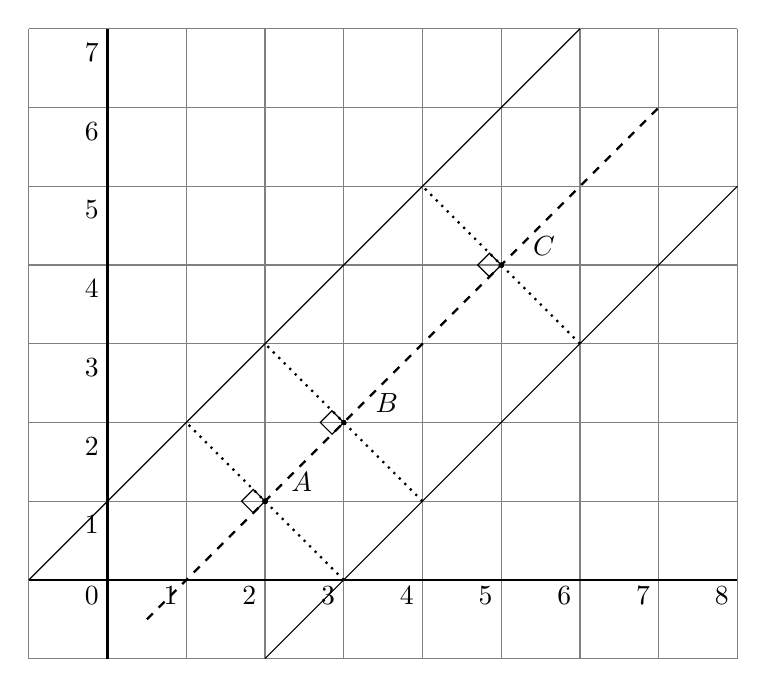
\begin{tikzpicture}[scale=1]
\draw[step=10mm,white!50!black,thin] (-1,-1) grid (8,7);
\draw[thick] (-1,0) -- (8,0);
\draw[thick] (0,-1) -- (0,7);
\foreach \x in {0,...,8}
  \node at (\x-.2,-.2) {\sm{\x}};
\foreach \y in {1,...,7}
  \node at (-.2,\y-.3) {\sm{\y}};
\draw (-1,0) -- (6,7);
\draw (2,-1) -- (8,5);
\draw[thick,dashed] (.5,-.5) -- (7,6);
\draw[thick,dotted] (3,0) -- (1,2);
\draw[thick,dotted] (4,1) -- (2,3);
\draw[thick,dotted] (6,3) -- (4,5);
\coordinate (A) at (2,1);
\node[above right,xshift=6pt] at (A) {$A$};
\coordinate (B) at (3,2);
\node[above right,xshift=8pt] at (B) {$B$};
\coordinate (C) at (5,4);
\node[above right,xshift=8pt] at (C) {$C$};
\fill (A) circle (1.1pt);
\fill (B) circle (1pt);
\fill (C) circle (1pt);
\draw[rotate=135] (A) rectangle +(6pt,6pt);
\draw[rotate=135] (B) rectangle +(6pt,6pt);
\draw[rotate=135] (C) rectangle +(6pt,6pt);
\end{tikzpicture}
\end{center}

%%%%%%%%%%%%%%%%%%%%%%%%%%%%%%%%%%%%%%%%%%%%%%%%%%%%%%%%%%%%%%%%%%
%%%%%%%%%%%%%%%%%%%%%%%%%%%%%%%%%%%%%%%%%%%%%%%%%%%%%%%%%%%%%%%%%%
%%%%%%%%%%%%%%%%%%%%%%%%%%%%%%%%%%%%%%%%%%%%%%%%%%%%%%%%%%%%%%%%%%

\subsection{A locus that is a line segment}

\begin{wrapfigure}[6]{r}{.33\textwidth}
% Axiom 1
\begin{center}
\vspace{-3ex}
\begin{tikzpicture}[scale=.9]
\coordinate (P1) at (3,6);
\coordinate (P2) at (4,3);
\fill (P1) circle (1.5pt) node[below left] {$P_1$};
\fill (P2) circle (1.5pt) node[below left] {$P_2$};
\draw[thick,dashed] ($(P1)!-.2!(P2)$) -- ($(P1)!1.5!(P2)$);
\draw[very thick,dotted,->,bend left=35] (5,5) to (2,4);
\end{tikzpicture}
\end{center}
\end{wrapfigure}
Consider Axiom 1: Given two points $P_1,P_2$, there is a single fold $l$ that passes through both points. 

Take a sheet of paper and perform the following operations:
\begin{itemize}
\item Choose two points and label them $P_1,P_2$.
\item Construct a fold that passes through both points.
\item Mark the line constructed by the fold and label it $l$.
\end{itemize}

Let us consider first only points that lie on the line segment $\overline{P_1P_2}$. Try to express a properties that characterizes all the points on the segment. Hint: Choose an arbitrary point on $\overline{P_1P_2}$. What is the sum of the distances from $P_1$ and $P_2$?

Are there other points in the plane not on $\overline{P_1P_2}$ that satisfy the same property? Justify your answer. Hint: The sum of the length of two sides of a triangle is always greater than the length of the third.

\begin{center}
\framebox[.9\textwidth]{\parbox{.85\textwidth}{
For an arbitrary point $A$ on $\overline{P_1P_2}$, $\overline{P_1P_2}= \overline{P_1A}+\overline{AP_2}$.
}}
\end{center}

\begin{center}
\framebox[.9\textwidth]{\parbox{.85\textwidth}{
The line segment $\overline{P_1P_2}$ is the geometric locus of all points the sum of whose distances from $P_1$ and $P_2$ is equal to the length of $\overline{P_1P_2}$.
}}
\end{center}

\begin{center}
\begin{tikzpicture}[scale=1.1]
\draw[step=10mm,white!50!black,thin] (-1,-1) grid (8,7);
\draw[thick] (-1,0) -- (8,0);
\draw[thick] (0,-1) -- (0,7);
\foreach \x in {0,...,8}
  \node at (\x-.2,-.2) {\sm{\x}};
\foreach \y in {1,...,7}
  \node at (-.2,\y-.3) {\sm{\y}};
\coordinate (P1) at (1,4);
\coordinate (P2) at ($(P1)+(-30:6)$);
\fill (P1) circle (1.5pt) node[below left] {$P_1$};
\fill (P2) circle (1.5pt) node[below left,xshift=-4pt] {$P_2$};
\draw[thick] (P1) -- (P2);
%\draw[thick,dashed] ($(P1)!-.4!(P2)$) -- ($(P1)!1.4!(P2)$);
\draw[<->] ($(P1)+(.2,.4)$) -- node[fill=white] {$a$} ($(P1)+(0,.4)+(-30:4)$);
\draw[<->] ($(P1)+(0,.4)+(-30:4)$) -- node[fill=white] {$b$}  ($(P1)+(0,.4)+(-30:6.2)$);
\node at (5.15,3.5) {$\overline{P_1P_2}=\!a+\!b$};
\fill ($(P1)+(-30:3.8)$) circle(1.5pt) node[below,yshift=-4pt] {$A$};
\end{tikzpicture}
\end{center}

Consider now the points on $l$ that are not on $\overline{P_1P_2}$. Try to find a property that characterizes all such points. Hint: Choose an arbitrary point $A$ on $l$ but not on $\overline{P_1P_2}$ and look at the difference between the lengths $\overline{AP_1}$ and $\overline{AP_2}$.

Are there other points on the plane not on $l$ that satisfy this property? Hint: The sum of the length of two sides of any triangle is always greater than the length of the third side.

\begin{center}
\begin{tikzpicture}[scale=1.2]
\draw[step=10mm,white!50!black,thin] (-1,-1) grid (8,7);
\draw[thick] (-1,0) -- (8,0);
\draw[thick] (0,-1) -- (0,7);
\foreach \x in {0,...,8}
  \node at (\x-.2,-.2) {\sm{\x}};
\foreach \y in {1,...,7}
  \node at (-.2,\y-.3) {\sm{\y}};
\coordinate (P1) at (1,4);
\coordinate (P2) at ($(P1)+(-30:4)$);
\fill (P1) circle (1.5pt) node[below left] {$P_1$};
\fill (P2) circle (1.5pt) node[below left,xshift=-4pt] {$P_2$};
\draw[thick] (P1) -- (P2);
\coordinate (p) at ($(P1)+(-30:6)$);
\draw[thick,dashed] (P2) -- (p);
\fill (p) circle (1.5pt) node[below] {$A$};
%\draw[thick,dashed] ($(P1)!-.4!(P2)$) -- ($(P1)!1.4!(P2)$);
\draw[<->] ($(P1)+(.2,.4)$) -- node[fill=white] {$a$} ($(P1)+(0,.4)+(-30:6.15)$);
\draw[<->] ($(P1)+(0,.8)+(-30:4.3)$) -- node[fill=white] {$b$}  ($(P1)+(0,.8)+(-30:6.2)$);
\node at (5.15,3.5) {$\overline{P_1P_2}=\!a-\!b$};
\end{tikzpicture}
\end{center}

We have found two properties one of which is satisfied by every point on $l$. Can you characterize the geometric locus defined by $l$?

\begin{center}
\framebox[.9\textwidth]{\parbox{.85\textwidth}{
\textbf{Conclusion}\\
$l$, the line constructed by the fold, is the geometric locus of all points $A$ such that the sum or difference of the lengths of $A$ from $P_1$ and $P_2$ is equal to the length of $\overline{P_1P_2}$.
}}
\end{center}
%%%%%%%%%%%%%%%%%%%%%%%%%%%%%%%%%%%%%%%%%%%%%%%%%%%%%%%%%%%%%%%%%%
%%%%%%%%%%%%%%%%%%%%%%%%%%%%%%%%%%%%%%%%%%%%%%%%%%%%%%%%%%%%%%%%%%
%%%%%%%%%%%%%%%%%%%%%%%%%%%%%%%%%%%%%%%%%%%%%%%%%%%%%%%%%%%%%%%%%%

\subsection{Loci appearing in Axiom 5}

\subsubsection{The circle as a locus}


\begin{wrapfigure}[5]{r}{.33\textwidth}
\begin{center}
\vspace{-6ex}
\begin{tikzpicture}[scale=1]
\coordinate (P1) at (1,4);
\coordinate (P2) at (4,3);
\fill (P1) circle (1.5pt) node[above left] {$P_1$};
\fill (P2) circle (1.5pt) node[below right] {$P_2$};
\draw[very thick,dotted] (P1) -- node[fill=white] {$a$} (P2);
\draw[thick,dashed] (0,1) -- (5,3.5);
\coordinate (P1a) at (3,0);
\fill (P1a) circle (1.5pt) node[below right,yshift=-2pt] {$P_1'$};
\draw[very thick, dotted] (P2) -- node[fill=white] {$a$} (P1a);
\draw[very thick,dotted,bend right=30,->] ($(P1)+(-.1,-.2)$) to ($(P1a)+(-.2,.1)$);
\end{tikzpicture}
\end{center}
\end{wrapfigure}
Take a sheet of paper and perform the following actions:
\begin{itemize}
\item Mark two points $P_1,P_2$.
\item Construct a fold through $P_2$ but don't open the paper.
\item Mark the point $P_1'$ that $P_1$ lands on. Tip: make a hole through the paper at $P_1$ to simplify marking $P_1'$.
\item Explain why the distance from $P_1$ to $P_2$ is equal to the distance from $P_1'$ to $P_2$ (both are labeled $a$ in the diagram).
\item Open the paper and perform the actions again and again with  different folds.
\end{itemize}
What is the common property of all the new points that are constructed?
\begin{center}
\begin{tikzpicture}[scale=1.1]
\draw[step=10mm,white!50!black,thin] (-1,-1) grid (8,7);
\draw[thick] (-1,0) -- (8,0);
\draw[thick] (0,-1) -- (0,7);
\foreach \x in {0,...,8}
  \node at (\x-.2,-.2) {\sm{\x}};
\foreach \y in {1,...,7}
  \node at (-.2,\y-.3) {\sm{\y}};
\coordinate (P1) at (1,4);
\coordinate (P2) at (4,3);
\fill (P1) circle (1.5pt) node[above left] {$P_1$};
\fill (P2) circle (1.5pt) node[below right] {$P_2$};
\draw[very thick,dotted] (P1) -- node[fill=white] {$r$} (P2);
\draw[thick,dashed] (0,1) -- (8,5);
\coordinate (P1a) at (3,0);
\fill (P1a) circle (1.5pt) node[below right,yshift=-2pt] {$P_1'$};
\draw[very thick, dotted] (P2) -- node[fill=white] {$r$} (P1a);
%\draw (P1) -- (P1a);
\draw[thick,dashed] ($(5,0)!1.1!(3,6)$) -- ($(3,6)!1.1!(5,0)$);
\coordinate (C) at ($(5,0)!(P1)!(3,6)$);
\coordinate (P1b) at ($(P1)!2!(C)$);
\fill (P1b) circle (1.5pt) node[right, xshift=4pt] {$P_1''$};
%\draw (P1) -- (P1b);
\draw[very thick,dotted] (P2) -- node[fill=white] {$r$} (P1b);
\draw[very thick,dotted,bend left=30,->] ($(P1)+(.1,.2)$) to ($(P1b)+(-.1,.1)$);
\draw[very thick,dotted,bend right=30,->] ($(P1)+(-.1,-.2)$) to ($(P1a)+(-.2,.1)$);
\end{tikzpicture}
\end{center}

\begin{center}
\framebox[.9\textwidth]{\parbox{.85\textwidth}{
All the points are the same distance from $P_2$; this distance is the length of $\overline{P_1P_2}$.
}}
\end{center}

Looking at the paper, what figure is formed by the new points?

Observe the Geogebra application called \texttt{circle.ggb}. Given points $P,Q$, the slider can be used to change the slope of the fold that passes through point $Q$. $P'$ is the reflection of point $P$ around the fold and its place will change as the slope of the fold is changed. If you check the box labeled ``Show trace of $P_1'$'', you can see all the reflected points.\footnote{The track can be erased by pressing ``Ctrl-F''.}
\begin{center}
\begin{tikzpicture}[scale=1.1]
\draw[step=10mm,white!50!black,thin] (-1,-1) grid (8,7);
\draw[thick] (-1,0) -- (8,0);
\draw[thick] (0,-1) -- (0,7);
\foreach \x in {0,...,8}
  \node at (\x-.2,-.2) {\sm{\x}};
\foreach \y in {1,...,7}
  \node at (-.2,\y-.3) {\sm{\y}};
\coordinate (P1) at (1,4);
\coordinate (P2) at (4,3);
\fill (P1) circle (1.5pt) node[above left] {$P_1$};
\fill (P2) circle (1.5pt) node[below right,xshift=2pt] {$P_2$};
\draw[very thick,dotted] (P1) -- node[fill=white] {$r$} (P2);

\draw[thick,dashed] (0,1) -- (8,5);
\coordinate (P1a) at (3,0);
\fill (P1a) circle (1.5pt) node[below right,yshift=-2pt] {$P_1'$};
\draw[very thick, dotted] (P2) -- node[fill=white] {$r$} (P1a);
%\draw (P1) -- (P1a);
\draw[thick,dashed] ($(5,0)!1.1!(3,6)$) -- ($(3,6)!1.1!(5,0)$);
\coordinate (C) at ($(5,0)!(P1)!(3,6)$);
\coordinate (P1b) at ($(P1)!2!(C)$);
\fill (P1b) circle (1.5pt) node[right, xshift=4pt] {$P_1''$};
%\draw (P1) -- (P1b);
\draw[very thick,dotted] (P2) -- node[fill=white] {$r$} (P1b);
\node[draw,circle through=(P1)] at (P2) {};
\end{tikzpicture}
\end{center}
The reflected points form a circle. What is its center and radius? 

Could there be reflected points not on the circle, that is, inside or outside the circle? Explain.

What is the geometric locus of all points at a fixed distance from a given point?


\begin{center}
\framebox[.9\textwidth]{\parbox{.85\textwidth}{
The geometric locus of points at a fixed distance from a given point is a circle.
}}
\end{center}

%%%%%%%%%%%%%%%%%%%%%%%%%%%%%%%%%%%%%%%%%%%%%%%%%%%%%%%%%%%%%%%%%%
%%%%%%%%%%%%%%%%%%%%%%%%%%%%%%%%%%%%%%%%%%%%%%%%%%%%%%%%%%%%%%%%%%
%%%%%%%%%%%%%%%%%%%%%%%%%%%%%%%%%%%%%%%%%%%%%%%%%%%%%%%%%%%%%%%%%%

\subsubsection{Individual points are loci}

% Axiom 5
\begin{wrapfigure}[7]{r}{.33\textwidth}
\begin{center}
\vspace{-6ex}
\begin{tikzpicture}[scale=.8]
\coordinate (P1) at (1,4);
\coordinate (P2) at (4,3);
\fill (P1) circle (1.5pt) node[above left] {$P_1$};
\fill (P2) circle (1.5pt) node[below right] {$P_2$};
\draw[thick,dashed] (2.5,-1.5) -- (4.6,4.8); %($(3,0)!-.15!(5,6)$) -- (5,6);
\draw[thick] (1,-1) -- node[above] {$l$} ($(1,-1)!1.15!(7,2)$);
\coordinate (P3) at (7,2);
\fill (P3) circle (1.5pt) node[below right] {$P_1'$};
\draw[->,very thick,dotted,bend left=40] ($(P1)+(.2,.15)$) to ($(P3)+(-.2,.15)$);
\end{tikzpicture}
\end{center}
\end{wrapfigure}
Consider Axiom $5$: given two points $P_1,P_2$ and line $l$, there is a fold that places $P_1$ onto $l$ and passes through $P_2$.

Previously we saw that for any fold that passes through $P_2$, the possible reflections for $P_1$ form a circle whose center is $P_2$ and whose radius is the length of the line segment $\overline{P_1P_2}$. Axiom~$5$ adds a condition.

\begin{itemize}
\item What is the condition?
\item Of all the folds that constructed the circle, how may can possibly place $P_1$ onto the line $l$? There are three cases because the $l$ can intersect the circle in zero, one or two points. Use the Geogebra application to help answer this question.
\end{itemize}

\begin{center}
\begin{tikzpicture}[scale=.9]
\draw[step=10mm,white!50!black,thin] (-1,-1) grid (9,9);
\draw[thick] (-1,0) -- (9,0);
\draw[thick] (0,-1) -- (0,9);
\foreach \x in {0,...,9}
  \node at (\x-.2,-.2) {\sm{\x}};
\foreach \y in {1,...,9}
  \node at (-.2,\y-.3) {\sm{\y}};
\coordinate (L1a) at (-1,3.5);
\coordinate (L1b) at (8,-1);
\draw[name path=L1] (L1a) -- node[below,xshift=8pt,yshift=-8pt] {$l$} (L1b);
\coordinate (P1) at (2,8);
\fill (P1) circle (2pt) node[above left] {$P$};
\coordinate (P2) at (4,4);
\fill (P2) circle (2pt) node[above left,yshift=4pt] {$Q$};
\node[very thick,dotted,draw, name path = circle] at (P2)
    [circle through = (P1)] {};

\path [name intersections = {of = circle and L1, by = {P1P,P1PP}}];
\fill (P1P) circle (2pt) node[above left,xshift=-2pt,yshift=4pt] {$P''$};
\fill (P1PP) circle (2pt) node[above left,yshift=6pt] {$P'$};

\coordinate (f1) at (0,6);
\draw[thick,dashed] ($(f1)!-.25!(P2)$) -- node[very near end,above] {$f_2$} ($(f1)!2.25!(P2)$);
\coordinate (f2) at (0,2);
\draw[thick,dashed] ($(f2)!-.25!(P2)$) -- node[very near end,below,yshift=-2pt] {$f_1$} ($(f2)!2.25!(P2)$);

\draw[very thick,dotted,->,bend left=50] (2.2,7.8) to (-.2,3.2);
\draw[very thick,dotted,->,bend left=50] (2.4,7.85) to (6.1,.2);
\end{tikzpicture}
\end{center}
\textbf{Explanation of the Geogebra application} Given points $P,Q$ and line $l$, there are two folds $f_1,f_2$ through $Q$ that place $P$ onto $l$ at $P',P''$. In the previous application we saw that the geometric locus of the reflected points is a circle whose center is $Q$ and whose radius is the length of $\overline{PQ}$. The point $P',P''$ define the possible folds. Note that there will be no folds if the line $l$ does not intersect the circle and there will be one fold if the line is tangent to the circle.


Axiom $5$ describes the geometric locus of points on line $l$ whose distance from $P_2$ is the length of the line segment $\overline{P_1P_2}$. What is the form of the geometric locus in each of the cases described above?
\begin{center}
\framebox[.9\textwidth]{\parbox{.85\textwidth}{
Answers: Zero, one or two points depending on the number of intersections of $l$ with the circle formed by the points at distance $\overline{P_1P_2}$ from $P_2$.
}}
\end{center}

%%%%%%%%%%%%%%%%%%%%%%%%%%%%%%%%%%%%%%%%%%%%%%%%%%%%%%%%%%%%%%%%%%
%%%%%%%%%%%%%%%%%%%%%%%%%%%%%%%%%%%%%%%%%%%%%%%%%%%%%%%%%%%%%%%%%%
%%%%%%%%%%%%%%%%%%%%%%%%%%%%%%%%%%%%%%%%%%%%%%%%%%%%%%%%%%%%%%%%%%

\subsection{Loci appearing in Axiom 6}

\subsubsection{The parabola as a locus}

\begin{wrapfigure}[2]{r}{.4\textwidth}
\begin{center}
\vspace{-6ex}
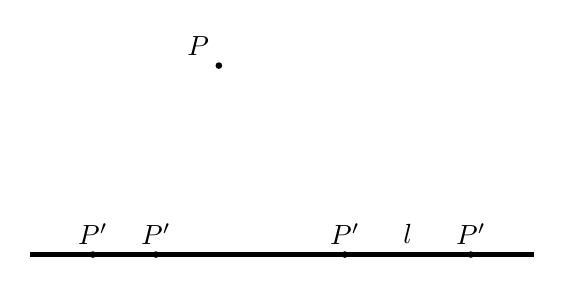
\begin{tikzpicture}[scale=.8]
\draw[ultra thick] (0,0) -- node[above, near end] {$l$} (8,0);
\fill (3,3) circle (1.5pt) node[above left] {$P$};
\foreach \x in {1,2,5,7}
  \fill (\x,0) circle (1.5pt) node[above] {$P'$};
\end{tikzpicture}
\end{center}
\end{wrapfigure}
Take a sheet of paper and perform the following actions:
\begin{itemize}
\item Mark the line $l$ that is one edge of the paper.
\item Choose a point $P$ \emph{near} $l$ and a point $P'$ \emph{on} $l$.
\item Fold the paper so that $P'$ is place on $P$.
\item Open the paper and perform this action again and again for different positions of $P'$ on $l$.
\end{itemize}
Open the paper and observe the form created by the multiple folds. If necessary, perform additional folds until the form becomes clear.
\begin{center}
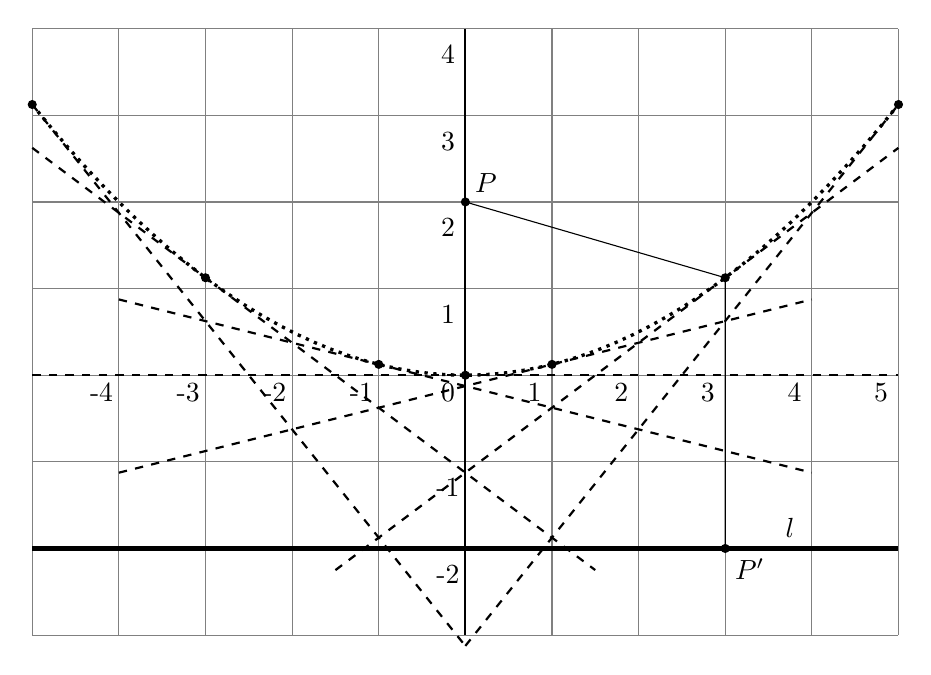
\begin{tikzpicture}[scale=1.1]
\draw[step=10mm,white!50!black,thin] (-2,-1) grid (8,6);
\draw[ultra thick] (-2,0) -- node[above, very near end] {$l$} (8,0);
\draw[thick,dashed] (-2,2) -- (8,2);
\draw[thick] (3,-1) -- (3,6);
\foreach \x in {-4,...,5}
  \node at (\x+3-.2,2-.2) {\sm{\x}};
\foreach \y in {-2,-1}
  \node at (3-.2,\y+2-.3) {\sm{\y}};
\foreach \y in {1,...,4}
  \node at (3-.2,\y+2-.3) {\sm{\y}};
\draw[domain=-5:5,samples=50,very thick,dotted,xshift=3cm,yshift=2cm] plot (\x,{(\x*\x)/8});
\coordinate (focus) at (3,4);
\fill (focus) circle(1.5pt) node[above right] {$P$};
\coordinate (pp) at (3+3,0);
\fill (pp) circle(1.5pt) node[below right] {$P'$};

\coordinate (p0) at (0+3,0+2);
\fill (p0) circle(1.5pt);
\coordinate (p1) at (1+3,.125+2);
\fill (p1) circle(1.5pt);
\coordinate (p3) at (3+3,1.125+2);
\fill (p3) circle(1.5pt);
\coordinate (p5) at (5+3,3.125+2);
\fill (p5) circle(1.5pt);

\draw (focus) -- (p3) -- (pp);


\coordinate (mp1) at (-1+3,.125+2);
\fill (mp1) circle(1.5pt);
\coordinate (mp3) at (-3+3,1.125+2);
\fill (mp3) circle(1.5pt);
\coordinate (mp5) at (-5+3,3.125+2);
\fill (mp5) circle(1.5pt);

\draw[domain=-4:4,samples=50,thick,dashed,xshift=3cm,yshift=2cm] plot (\x,{.125*(2*\x-1)});

\draw[domain=-1.5:5,samples=50,thick,dashed,xshift=3cm,yshift=2cm] plot (\x,{.375*(2*\x-3)});

\draw[domain=0:5,samples=50,thick,dashed,xshift=3cm,yshift=2cm] plot (\x,{.625*(2*\x-5)});

\draw[domain=-4:4,samples=50,thick,dashed,xshift=3cm,yshift=2cm] plot (\x,{-.125*(2*\x+1)});

\draw[domain=-5:1.5,samples=50,thick,dashed,xshift=3cm,yshift=2cm] plot (\x,{-.375*(2*\x+3)});

\draw[domain=-5:0,samples=50,thick,dashed,xshift=3cm,yshift=2cm] plot (\x,{-.625*(2*\x+5)});

\end{tikzpicture}
\end{center}
Use the Geogebra application \texttt{parabola.ggb} and select ``Show trace of $P$'' and move the slider to change the position of the point $P$. Then select ``Show locus'' to see the parabola formed by the positions of point $P$.

What do you think is the relationship between the folds and the parabola? Later we will prove that the folds are tangents to the parabola. 

Write down the definition of a parabola? Determine the focus and directrix for the parabola defined by the folds.


\textbf{How is the parabola formed?}
\begin{itemize}
\item Choose a point $P'$ on $l$ on the sheet of paper you have been using. Fold the paper so that $P'$ is placed onto $P$. Mark the line created by the fold and label it $l'$.
\item Construct a perpendicular to $l$ through the point $P'$. Label the intersection of the perpendicular and $l'$.
\item Show by folding that that $\overline{AP}=\overline{AP'}$. What can you conclude about the point $A$?
\end{itemize}
\begin{center}
\framebox[.9\textwidth]{\parbox{.85\textwidth}{
The distance of $A$ from $P$ is equal to the distance from $A$ to $l$. Therefore, $A$ is a point on the parabola whose focus is $P$ and whose directrix is $l$.
}}
\end{center}

\begin{center}
\begin{tikzpicture}[scale=1]
\draw[step=10mm,white!50!black,thin] (-1,-1) grid (8,7);
\draw[ultra thick] (-1,0) -- node[above, very near end] {$l$} (8,0);
\draw[thick] (0,-1) -- (0,7);
\foreach \x in {0,...,8}
  \node at (\x-.2,-.2) {\sm{\x}};
\foreach \y in {1,...,7}
  \node at (-.2,\y-.3) {\sm{\y}};
\coordinate (A) at (1,4);
\coordinate (P) at (5,2);
\coordinate (PP) at (1,0);
\fill (A) circle (1.5pt) node[above right] {$A$};
\fill (P) circle (1.5pt) node[below right] {$P$};
\fill (PP) circle (1.5pt) node[below left] {$P'$};
\draw (PP) -- (A) -- (P);
\draw[thick] (PP) rectangle +(6pt,6pt);
\draw[thick,dashed] ($(A)!-.5!(4,-1)$) -- node [right,xshift=6pt,yshift=-4pt] {$l'$} (4,-1);
\end{tikzpicture}
\end{center}

If we take into consideration all the possible folds, we obtain a parabola.
\begin{center}
\framebox[.9\textwidth]{\parbox{.85\textwidth}{
The geometric locus of all points equidistant from a given point (the focus) and a given line (the directrix) is a parabola.
}}
\end{center}

\begin{center}
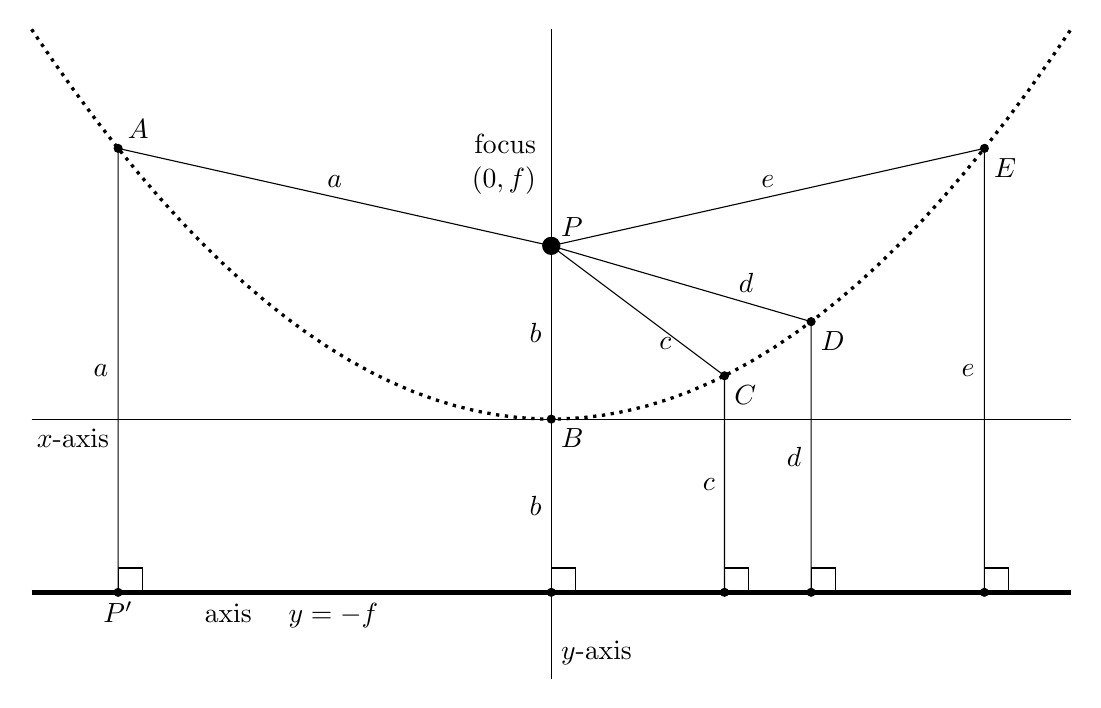
\begin{tikzpicture}[scale=1.1]
\draw (-6,0) -- node[very near start,below,xshift=-32pt] {$x$-axis} (6,0);
\draw (0,-3) -- node[very near start,right,yshift=-20pt] {$y$-axis} (0,4.5);
\draw[ultra thick] (-6,-2) -- node[near start,below] {axis $\quad y=-f$} (6,-2);
\draw[domain=-6:6,samples=50,very thick,dotted] plot (\x,{\x*\x/8});
\coordinate (F) at (0,2);
\fill (F) circle (3pt) node[above left,xshift=-2pt,yshift=15pt] {$(0,f)$} node[above left,xshift=-2pt,yshift=30pt] {focus} node[above right] {$P$};
\fill (0,0) circle (1.5pt) node[below right] {$B$};
\fill (0,-2) circle (1.5pt);
\fill (2,-2) circle (1.5pt);
\fill (3,-2) circle (1.5pt);
\fill (5,-2) circle (1.5pt);
\coordinate (FP) at (-5,-2);
\fill (FP) circle (1.5pt) node[below] {$P'$};
\coordinate (F1) at (2,.5);
\fill (F1) circle (1.5pt) node[below right] {$C$};
\coordinate (F2) at (3,1.125);
\fill (F2) circle (1.5pt) node[below right] {$D$};
\coordinate (F3) at (5,3.125);
\fill (F3) circle (1.5pt) node[below right] {$E$};
\coordinate (F4) at (-5,3.125);
\fill (F4) circle (1.5pt) node[above right] {$A$};
\draw (F) -- node[left] {$b$} (0,0) -- node[left] {$b$} (0,-2);
\draw (F) -- node[near end,left] {$c$} (F1) -- node[left] {$c$} (2,-2);
\draw (F) -- node[near end,above] {$d$} (F2) -- node[left] {$d$} (3,-2);
\draw (F) -- node[above] {$e$} (F3) -- node[left] {$e$} (5,-2);
\draw (F) -- node[above] {$a$} (F4) -- node[left] {$a$} (FP);
\draw (0,-2) rectangle +(8pt,8pt);
\draw (2,-2) rectangle +(8pt,8pt);
\draw (3,-2) rectangle +(8pt,8pt);
\draw (5,-2) rectangle +(8pt,8pt);
\draw (-5,-2) rectangle +(8pt,8pt);
\end{tikzpicture}
\end{center}

%%%%%%%%%%%%%%%%%%%%%%%%%%%%%%%%%%%%%%%%%%%%%%%%%%%%%%%%%%%%%%%%%%
%%%%%%%%%%%%%%%%%%%%%%%%%%%%%%%%%%%%%%%%%%%%%%%%%%%%%%%%%%%%%%%%%%
%%%%%%%%%%%%%%%%%%%%%%%%%%%%%%%%%%%%%%%%%%%%%%%%%%%%%%%%%%%%%%%%%%


\subsubsection{The tangent to a parabola}

Previously we saw that the set of folds that place a given point onto a given line forms a parabola. We now prove that each of these folds is a tangent to the parabola.
\begin{itemize}
\item Given a parabola with focus $P$ and directrix $l$, let $P'$ be a point on $l$. Prove that the fold that places $P$ onto $P'$ is the perpendicular bisector of the line segment $\overline{PP'}$. Hint: Prove that $\triangle APB \cong \triangle AP'B$.
\begin{center}
\begin{tikzpicture}[scale=.7]
\draw[ultra thick] (-6,-2) -- node[below,near end] {$l$}
(6,-2);
\draw[domain=-6:6,samples=50,very thick,dotted,name path=parb] plot (\x,{\x*\x/8});
\coordinate (F) at (0,2);
\fill (F) circle (2pt) node[above right] {$P$};
\coordinate (FP) at (-5,-2);
\fill (FP) circle (2pt) node[below] {$P'$};
\coordinate (F4) at (-5,3.125);
\draw[name path=perp,thick] (F) -- (FP);
\draw[thick,dashed,name path=fold] ($(F4)!-.4!(-2.5,0)$) --
($(F4)!1.8!(-2.5,0)$);
\path [name intersections = {of = fold and perp, by = {T}}];
\path [name intersections = {of = fold and parb, by = {Tan}}];
\fill (T) circle (2pt) node[below,xshift=-2pt,yshift=-3pt] {$B$};
\fill (Tan) circle (2pt) node[below left] {$A$};
\draw[thick,rotate=40] (T) rectangle +(8pt,8pt);
\draw (F) -- (Tan) -- (FP);
\end{tikzpicture}
\end{center}
\item Prove that the perpendicular bisector of the line segment connecting the focus with a point on the directrix is a tangent to the parabola.
\item Label the perpendicular bisector by $m$ and label its intersection with $\overline{PP'}$ by $B$.
\item Suppose that $m$ is not a tangent of the parabola. Then $m$ intersects the parabola in two different points, so there is a point $A'$ on $m$ that is distinct from $A$. Drop a perpendicular from $A'$ to $l$ and label its intersection with $l$ by $C$.
\item $A'$ is on the perpendicular bisector of $\overline{PP'}$ so $\overline{A'P}=\overline{A'P'}$ because $\triangle A'PB\cong \triangle A'P'B$.
\begin{center}
\begin{tikzpicture}[scale=.9]
\draw[ultra thick] (-6,-2) -- node[near end, below] {$l$} (6,-2);
\draw[domain=-5.5:5.5,samples=50,very thick,dotted] plot (\x,{\x*\x/8});
\coordinate (F) at (0,2);
\fill (F) circle (2pt) node[above right] {$P$};
\coordinate (FP) at (-3,-2);
\fill (FP) circle (1.5pt) node[below] {$P'$};
\coordinate (F4) at (-3,1.125);
\fill (F4) circle (1.5pt) node[above,yshift=2pt,xshift=2pt] {$A$};
\coordinate (F5) at (-5,2.775);
\fill (F5) circle (1.5pt) node[left,yshift=-4pt] {$A'$};
\coordinate (F5p) at (-5,-2);
\fill (F5p) circle (1.5pt) node[below] {$C$};
\draw (F) -- (F4) -- (FP);
%node[above] {$b$} (F4) -- node[left] {$b$} 
\draw (F) -- %node[above] {$c$} 
(F5);

\draw (F5) -- 
%node[left] {$d$}
 (F5p);
\draw[thick,dashed,name path=fold] ($(F4)+(140:4)$) -- (F4) -- node[below,xshift=-2pt,yshift=-2pt] {$m$} ($(F4)+(-40:5.1)$);
\draw (FP) rectangle +(8pt,8pt);
\draw (F5p) rectangle +(8pt,8pt);
\draw (F5) -- (FP);
\draw[name path=base] (F) -- (FP);
\path [name intersections = {of = base and fold, by = {G}}];
\fill (G) circle (1.5pt) node[below,yshift=-4pt] {$B$};
\draw[rotate=140] (G) rectangle +(6pt,6pt);
%\path (FP) -- node[left] {$c$} (F5);
%\path (F) -- node[below] {$a$} (G) -- node[below] {$a$} (FP);

% Draw tick marks
\coordinate(APP) at ($(F)!.5!(F5)$) ;
\draw (APP) -- ($(APP)!1mm!-90:(F)$);
\draw (APP) -- ($(APP)!1mm!90:(F)$);
\coordinate(APPP) at ($(F5)!.5!(FP)$) ;
\draw (APPP) -- ($(APPP)!1mm!-90:(F5)$);
\draw (APPP) -- ($(APPP)!1mm!90:(F5)$);

\coordinate(AP1) at ($(F)!.48!(F4)$) ;
\draw (AP1) -- ($(AP1)!1mm!-90:(F)$);
\draw (AP1) -- ($(AP1)!1mm!90:(F)$);
\coordinate(AP2) at ($(F)!.52!(F4)$) ;
\draw (AP2) -- ($(AP2)!1mm!-90:(F)$);
\draw (AP2) -- ($(AP2)!1mm!90:(F)$);

\coordinate(AAP1) at ($(F4)!.48!(FP)$) ;
\draw (AAP1) -- ($(AAP1)!1mm!-90:(F4)$);
\draw (AAP1) -- ($(AAP1)!1mm!90:(F4)$);
\coordinate(AAP2) at ($(F4)!.52!(FP)$) ;
\draw (AAP2) -- ($(AAP2)!1mm!-90:(F4)$);
\draw (AAP2) -- ($(AAP2)!1mm!90:(F4)$);
\end{tikzpicture}
\end{center}
\item $A'$ is on the parabola so $\overline{A'P}=\overline{A'C}$ and $l\perp \overline{A'C}$. It follows that $\overline{A'P'}=\overline{A'C}$.
\item It follows that in the right triangle $\triangle A'CP'$, the length of the side $\overline{A'C}$ is equal to the length of the hypotenuse $\overline{A'P'}$ which is impossible.
\item We conclude that $m$ cannot intersect the parabola in more than one point so it is a tangent to the parabola.
\end{itemize}

\begin{center}
\framebox[.9\textwidth]{\parbox{.85\textwidth}{
The perpendicular bisector of the line segment connecting the focus of a parabola and a point on the directrix is a tangent to the parabola.
}}
\end{center}

%%%%%%%%%%%%%%%%%%%%%%%%%%%%%%%%%%%%%%%%%%%%%%%%%%%%%%%%%%%%%%%%%%
%%%%%%%%%%%%%%%%%%%%%%%%%%%%%%%%%%%%%%%%%%%%%%%%%%%%%%%%%%%%%%%%%%
%%%%%%%%%%%%%%%%%%%%%%%%%%%%%%%%%%%%%%%%%%%%%%%%%%%%%%%%%%%%%%%%%%


\subsection{The locus described by Axiom 6}

% Axiom 6
\begin{wrapfigure}[8]{r}{.5\textwidth}
\begin{center}
\vspace{-8ex}
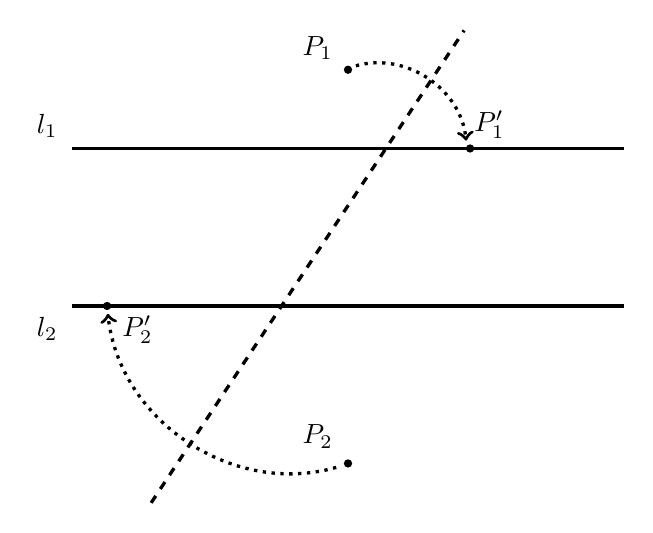
\begin{tikzpicture}[scale=.5]
\coordinate (P1) at (0,4);
\fill (P1) circle (3pt) node[above left,xshift=-2pt] {$P_1$};
\coordinate (P2) at (0,-6);
\fill (P2) circle (3pt) node[above left,xshift=-2pt,yshift=2pt] {$P_2$};
\coordinate (P1P) at (3.1,2);
\fill (P1P) circle (3pt) node[above right,xshift=-2pt] {$P_1'$};
\coordinate (P2P) at (-6.12,-2);
\fill (P2P) circle (3pt) node[below right,xshift=2pt] {$P_2'$};
\draw[very thick] (-7,2) -- node[very near start,above,xshift=-34pt] {$l_1$} (7,2);
\draw[very thick] (-7,-2) -- node[very near start,below,xshift=-34pt] {$l_2$} (7,-2);
\draw[very thick,dashed] (-5,-7) -- (2.95,5);
\draw[very thick,dotted,->,bend left=50] (.2,4.1) to (3,2.2);
\draw[very thick,dotted,->,bend left=50] (-.3,-6.1) to (-6.1,-2.2);
\end{tikzpicture}
\end{center}
\end{wrapfigure}
Consider Axiom $6$: Given two points $P_1,P_2$ and two lines $l_1,l_2$, there is a fold that places $P_1$ on $l_1$ and $P_2$ on $l_2$.

We saw that the set of folds that place a point $P$ on a line $l$ create a parabola. In addition we proved that each fold is a tangent to the parabola. Therefore, the folds that place $P_i$ on $l_i$, $i=1,2$ are the tangents to the parabolas whose foci are $P_i$ and whose directrices are $l_i$. 
%\begin{center}
%\begin{tikzpicture}[scale=1.2]
%\draw[step=10mm,white!50!black,thin] (-2,-1) grid (8,6);
%\draw[ultra thick] (-2,0) -- node[above, very near end] {$l$} (8,0);
%\draw[thick,dashed] (-2,2) -- (8,2);
%\draw[thick] (3,-1) -- (3,6);
%\foreach \x in {-4,...,5}
%  \node at (\x+3-.2,2-.2) {\sm{\x}};
%\foreach \y in {-2,-1}
%  \node at (3-.2,\y+2-.3) {\sm{\y}};
%\foreach \y in {1,...,4}
%  \node at (3-.2,\y+2-.3) {\sm{\y}};
%\draw[domain=-5:5,samples=50,very thick,dotted,xshift=3cm,yshift=2cm] plot (\x,{(\x*\x)/8});
%\coordinate (focus) at (3,4);
%\fill (focus) circle(1.5pt) node[above right] {$P$};
%\coordinate (pp) at (3+3,0);
%\fill (pp) circle(1.5pt) node[below right] {$P'$};
%\coordinate (p0) at (0+3,0+2);
%\fill (p0) circle(1.5pt);
%\coordinate (p1) at (1+3,.125+2);
%\fill (p1) circle(1.5pt);
%\coordinate (p3) at (3+3,1.125+2);
%\fill (p3) circle(1.5pt);
%\coordinate (p5) at (5+3,3.125+2);
%\fill (p5) circle(1.5pt);
%\draw (focus) -- (p3) -- (pp);
%\coordinate (mp1) at (-1+3,.125+2);
%\fill (mp1) circle(1.5pt);
%\coordinate (mp3) at (-3+3,1.125+2);
%\fill (mp3) circle(1.5pt);
%\coordinate (mp5) at (-5+3,3.125+2);
%\fill (mp5) circle(1.5pt);
%\draw[domain=-4:4,samples=50,thick,dashed,xshift=3cm,yshift=2cm] plot (\x,{.125*(2*\x-1)});
%\draw[domain=-1.5:5,samples=50,thick,dashed,xshift=3cm,yshift=2cm] plot (\x,{.375*(2*\x-3)});
%\draw[domain=0:5,samples=50,thick,dashed,xshift=3cm,yshift=2cm] plot (\x,{.625*(2*\x-5)});
%\draw[domain=-4:4,samples=50,thick,dashed,xshift=3cm,yshift=2cm] plot (\x,{-.125*(2*\x+1)});
%\draw[domain=-5:1.5,samples=50,thick,dashed,xshift=3cm,yshift=2cm] plot (\x,{-.375*(2*\x+3)});
%\draw[domain=-5:0,samples=50,thick,dashed,xshift=3cm,yshift=2cm] plot (\x,{-.625*(2*\x+5)});
%\end{tikzpicture}
%\end{center}

\newpage

How can a fold simultaneously satisfy these two conditions? 

The fold must be a tangent of both parabolas!

%\begin{wrapfigure}[8]{r}{.5\textwidth}
\begin{center}
%\vspace{-2ex}
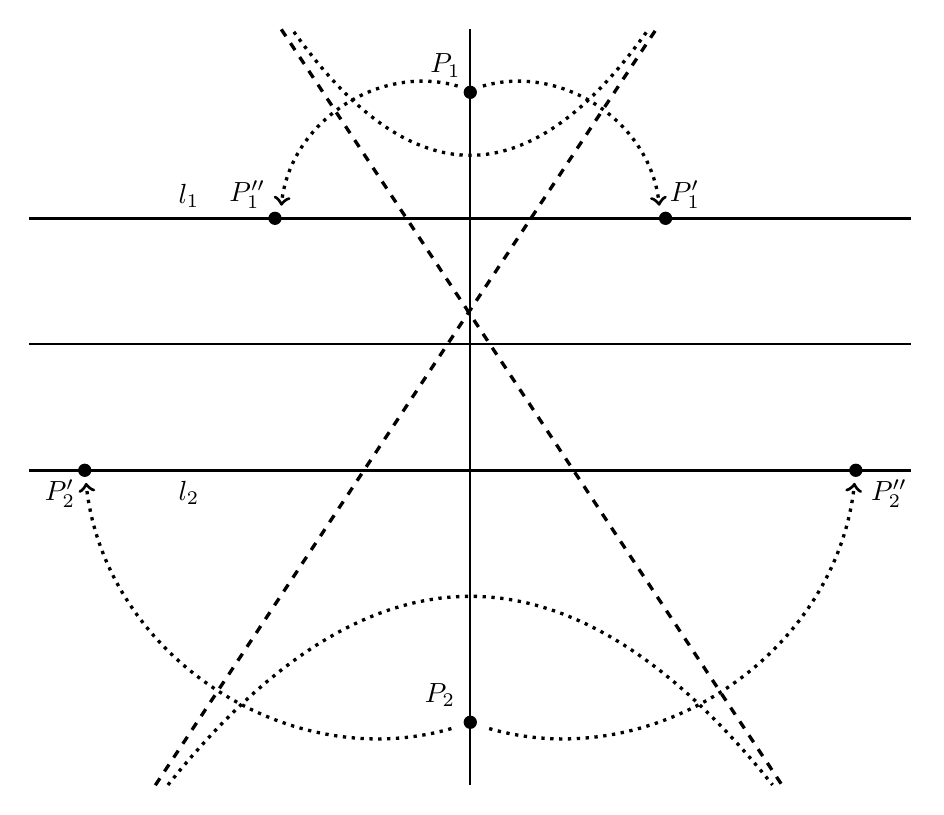
\begin{tikzpicture}[scale=.8]
\draw[thick] (-7,0) -- (7,0);
\draw[thick] (0,-7) -- (0,5);
\coordinate (P1) at (0,4);
\fill (P1) circle (3pt) node[above left,xshift=0pt,yshift=2pt] {$P_1$};
\coordinate (P2) at (0,-6);
\fill (P2) circle (3pt) node[above left,xshift=-2pt,yshift=2pt] {$P_2$};
\coordinate (P1P) at (3.1,2);
\fill (P1P) circle (3pt) node[above right,xshift=-2pt] {$P_1'$};
\coordinate (P2P) at (-6.12,-2);
\fill (P2P) circle (3pt) node[below left,xshift=0pt] {$P_2'$};
\coordinate (P1PP) at (-3.1,2);
\fill (P1PP) circle (3pt) node[above left,xshift=0pt] {$P_1''$};
\coordinate (P2PP) at (6.12,-2);
\fill (P2PP) circle (3pt) node[below right,xshift=2pt] {$P_2''$};
\draw[very thick] (-7,2) -- node[near start,above,xshift=-22pt] {$l_1$} (7,2);
\draw[very thick] (-7,-2) -- node[near start,below,xshift=-22pt] {$l_2$} (7,-2);
\draw[domain=-4.8:4.8,samples=50,very thick,dotted] plot (\x,{-.13*\x*\x-4});
\draw[domain=-2.8:2.8,samples=50,very thick,dotted] plot (\x,{.25*\x*\x+3});
\draw[very thick,dashed] (-5,-7) -- (2.95,5);
\draw[very thick,dashed] (-3,5) -- (4.95,-7);
\draw[very thick,dotted,->,bend left=50] (.2,4.1) to (3,2.2);
\draw[very thick,dotted,->,bend left=50] (-.3,-6.1) to (-6.1,-2.2);
\draw[very thick,dotted,->,bend right=50] (-.2,4.1) to (-3,2.2);
\draw[very thick,dotted,->,bend right=50] (.3,-6.1) to (6.1,-2.2);
\end{tikzpicture}
\end{center}
%\end{wrapfigure}
\begin{itemize}
\item Do all pairs of parabolas have a common tangent?
\item How many common tangents can a pair of parabolas have? See Appendix~\ref{a.parabola}.
\item What does it mean in terms of Axiom $6$ for a pair of parabolas to have more than one common tangent?
\end{itemize}
\begin{center}
\framebox[.9\textwidth]{\parbox{.85\textwidth}{
A fold resulting from Axiom $6$ is a common tangent to two parabolas with foci $P_1,P_1$ and directrices $l_1,l_2$.

Two parabolas can have zero, one, two or three common tangents.

Therefore, there can be zero, one, two or three folds satisfying Axiom 6 for any given $P_1, P_2, l_1, l_2$.
}}
\end{center}



%%%%%%%%%%%%%%%%%%%%%%%%%%%%%%%%%%%%%%%%%%%%%%%%%%%%%%%%%%%%%%%%%%
%%%%%%%%%%%%%%%%%%%%%%%%%%%%%%%%%%%%%%%%%%%%%%%%%%%%%%%%%%%%%%%%%%
%%%%%%%%%%%%%%%%%%%%%%%%%%%%%%%%%%%%%%%%%%%%%%%%%%%%%%%%%%%%%%%%%%

\subsection{The locus described by Axiom $4$}

\begin{wrapfigure}{r}{.4\textwidth}
% Axiom 4
\begin{center}
\vspace{-8ex}
\begin{tikzpicture}[scale=1]
\coordinate (L1a) at (3,2);
\coordinate (L1b) at (5,6);
\draw[thick] (L1a) -- node[very near start,right,yshift=-4pt] {$l$} ($(L1a)!1.15!(L1b)$);
\fill (3,5.5) circle (2pt) node[above right] {$P$};
\draw[thick,dashed] (2,6) -- (6,4);
\coordinate (intersection) at (4.4,4.8);
\draw[rotate=-30] (intersection) rectangle +(8pt,8pt);
\draw[very thick,dotted,->,bend left=50] (5.4,6.3) to (3.7,3);
\end{tikzpicture}
\end{center}
\end{wrapfigure}
\textbf{Axiom $4$} Given a point $P$ and a line $l$, there is a single fold perpendicular to $l$ that passes through $P$.
\begin{itemize}
\item Take a sheet of paper and mark an arbitrary point $P$ and an arbitrary line $l$.
\item Fold the paper so that the fold is perpendicular to $l$ and passes through $P$.
\item What is the geometric locus of the fold?
\end{itemize}
\vspace{-2ex}
\begin{center}
\framebox[.9\textwidth]{\parbox{.85\textwidth}{
The fold created by Axiom $4$ is the geometric locus of all points on the line perpendicular to $l$ and passing through $P$.
}}
\end{center}

\bigskip

\subsection{The locus described by Axiom $7$}


% Axiom 7
\begin{wrapfigure}[4]{r}{.4\textwidth}
\begin{center}
\vspace{-6ex}
\begin{tikzpicture}[scale=.6]
\coordinate (P1) at (5,3);
\fill (P1) circle (2pt) node[below left] {$P$};
\coordinate (P1P) at (2.75,5.25);
\fill (P1P) circle (2pt) node[left,xshift=-4pt] {$P'$};
\draw[very thick] (1,0) -- node[very near start,right,xshift=2pt] {$l_1$} (3,6);
\draw[very thick,name path=l2] (8,3) -- node[very near start,right,xshift=-2pt,yshift=6pt] {$l_2$} (5,6);
\draw[thick] ($(1,0)!-.15!(3,6)$) -- ($(1,0)!1.34!(3,6)$);
\draw[thick] ($(8,3)!-.3!(5,6)$) -- ($(8,3)!1.65!(5,6)$);
\draw[very thick,dashed,name path=fold] (-.5,-.25) -- (7.5,7.75);
\path [name intersections = {of = fold and l2, by = {perp}}];
\draw[rotate=-45] (perp) rectangle +(8pt,8pt);
\draw[very thick,dotted,->,bend right=50] (5.1,3.2) to (3,5.2);
\end{tikzpicture}
\end{center}
\end{wrapfigure}
\textbf{Axiom $7$} Given a point $P$ and two lines $l_1,l_2$, there is a fold that places $P$ onto $l_1$ and is perpendicular to $l_2$.
\begin{itemize}
\item Take a sheet of paper and mark a point $P$ and two lines $l_1,l_2$.
\item Fold the paper as described in Axiom $7$: a fold perpendicular to $l_2$ that places $P$ onto $l_1$.
\item Leave the paper folded and mark the point upon which $P$ is placed by $P'$.
\item Open the paper.
\end{itemize}
Explain why every point on the fold is equidistant from $p$ and $P'$.
Hint: Recall from Axiom $2$ and the activities that its geometric locus is the perpendicular bisector. 

What characterizes the set of points on the fold created by Axiom $7$?

What is the geometric locus described by those points?

\begin{center}
\framebox[.9\textwidth]{\parbox{.85\textwidth}{
The fold created by Axiom $7$ is the geometric locus of all points on the line perpendicular to $l_2$ and equidistant from $P$ and $P'$, the reflection of $P$ onto $l_1$.
}}
\end{center}

\begin{center}
\begin{tikzpicture}[scale=.9]
\draw[step=10mm,white!50!black,thin] (-1,-1) grid (9,8);
\draw[thick] (-1,0) -- (9,0);
\draw[thick] (0,-1) -- (0,8);
\foreach \x in {0,...,9}
  \node at (\x-.2,-.2) {\sm{\x}};
\foreach \y in {1,...,8}
  \node at (-.2,\y-.3) {\sm{\y}};
\coordinate (P1) at (5,3);
\fill (P1) circle (2pt) node[below left] {$P$};
\coordinate (P1P) at (2.75,5.25);
\fill (P1P) circle (2pt) node[left,xshift=-4pt] {$P'$};
\draw[very thick] (1,0) -- node[very near start,right,xshift=2pt] {$l_1$} (3,6);
\draw[very thick,name path=l2] (8,3) -- node[very near start,right,xshift=-2pt,yshift=6pt] {$l_2$} (5,6);
\draw[thick] ($(1,0)!-.15!(3,6)$) -- ($(1,0)!1.34!(3,6)$);
\draw[thick] ($(8,3)!-.3!(5,6)$) -- ($(8,3)!1.65!(5,6)$);
\draw[thick,dotted] ($(P1)!-.4!(P1P)$) -- node[very near start,below,yshift=-4pt] {$l_p$} ($(P1)!1.5!(P1P)$);
\draw[very thick,dashed,name path=fold] (-.5,-.25) -- node[very near end,above,xshift=4pt,yshift=6pt] {$l$} (7.5,7.75);
\coordinate(a) at ($(-.5,-.25)!.39!(7.5,7.75)$);
\fill (a) circle (2pt);
\draw (P1) -- node[below] {$a$} (a) -- node[left,near start] {$a$} (P1P);
\coordinate (mid) at ($(P1)!.5!(P1P)$);
\fill (mid) circle (2pt);
\path [name intersections = {of = fold and l2, by = {perp}}];
\draw[rotate=-45] (mid) rectangle +(8pt,8pt);
\draw[rotate=-45] (perp) rectangle +(8pt,8pt);
\draw[very thick,dotted,->,bend right=50] (5.1,3.2) to (3,5.2);
\end{tikzpicture}
\end{center}

